\section{Applications}

\subsection{Using StreamNet to cache TRIAS requests}

\begin{figure}[!ht]
        \begin{center}
                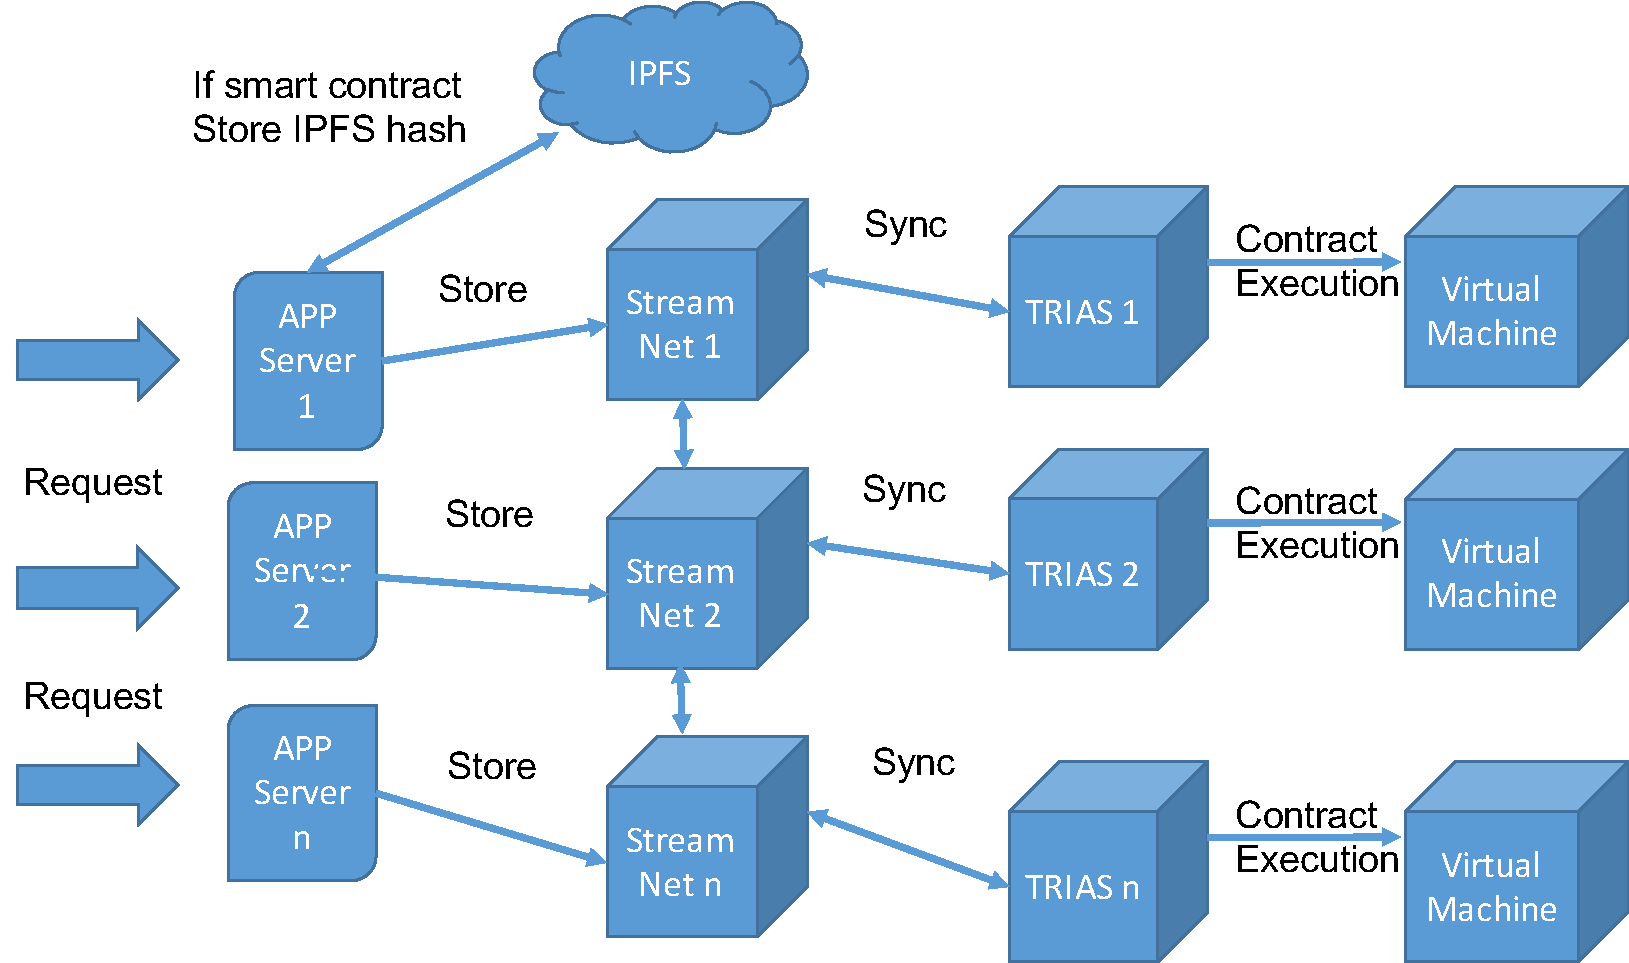
\includegraphics[width=0.50\textwidth]{figures/trias.pdf}
                \caption{StreamNet used for caching the TRIAS requests}
                \label{trias}
        \end{center}
\end{figure}

To avoid the selfish mining problem \cite{babaioff2012bitcoin, sapirshtein2016optimal}, there must be a way to let everyone in the network to know the request from the client side.
StreamNet can be used to cache and pre-confirm the information (including transactions and smart contracts) of other blockchain systems because of its high throughput.
$TRIAS$ \cite{trias18} as a cross-blockchain system can take advantage of this feature to achieve elasticity.
The structure is shown in Figure~\ref{trias}. 
There is a distributed APP server and each StreamNet deployment can have one APP server. 
APP server accept the TRIAS requests including the transaction and smart contract requests.
If the requests are transaction requests, APP server will send them directly to StreamNet in a batching mode (for instance, every 100 transactions is a batch) or a single mode.
If the requests are smart contract requests, APP server will send the info to IPFS to get a hash, then send this hash to StreamNet.
When the traffic is small, StreamNet can directly pass throught the content to $TRIAS$ after confirming it, 
When the traffic is large, StreamNet will continue to cache and pre-confirm the new blocks,
as $TRIAS$ is idle, it will pull the confirmed information from StreamNet and process it.

\subsection{Using StreamNet to rank TRIAS nodes in TEE environment}

\begin{figure}[!ht]
        \begin{center}
                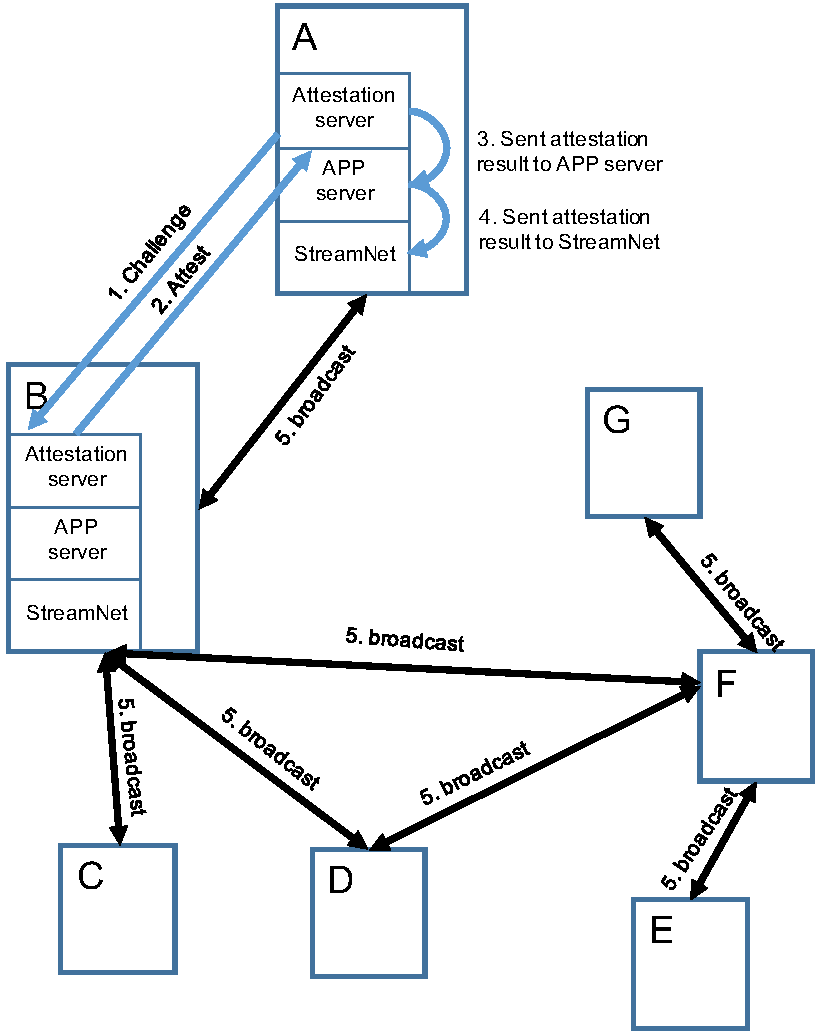
\includegraphics[width=0.40\textwidth]{figures/attestation.pdf}
                \caption{StreamNet involved in attestation.}
                \label{attestation}
        \end{center}
\end{figure}

\subsubsection{Attestation and synchronization of results}
Hybrid chain based systems usually use POW or POS to elect super nodes. 
Another thread of method utilized the trusted computing method \cite{ruan2017repcloud,ruan2014neuronvisor} to help elect super nodes. 
The general idea is, the blockchain system should run on the trusted computing environment (TEE),
and those who elected as the super node should prove that they are the most trustable nodes.
To achive this, there are attestation service periodically check the trusted status by attesting their neighbors. 
After the attestation result is collected, the attestation server will send this information to APP server, and it will be further directed to StreamNet.
By leveraging the gossip system of the StreamNet itself, these attestation information will be synchronized all through the network. The 5-step process is as Figure~\ref{attestation} shows.

\subsubsection{Global Tik Tok period}
One of the important issues in the attestation based reputation system in the open p2p network is that there is no common agreement of time.
In the private network, the typical solutions could be achived by using time oracle \cite{peng2010large} or TrueTime \cite{corbett2013spanner}.
Since StreamNet can provide with a total order, there is no need for TRIAS nodes to maintain a timer service.
StreamNet itself can provide with the concept of time (for instance the tik tok period of 1 hour).
The algorithm to determine current period and the blocks contained in current period is as Algorithm~\ref{algo:tik_tok} shows.
By using this algorithm, the attestation server will determin the current TikTok time $T_{current}$ and the last TikTok time $T_{last}$, and get all blocks between the time period. 
Once this step is done, the attestation server will send a TikTok time stamp to StreamNet for the next polling.
The $getTikTok()$ function in StreamNet tries to get the common consensus of the start point of a specific period.

\IncMargin{1em}
\begin{algorithm}
\SetKwData{Left}{left}\SetKwData{This}{this}\SetKwData{Up}{up}
\SetKwFunction{Union}{Union}\SetKwFunction{FindCompress}{FindCompress}
\SetKwInOut{Input}{input}\SetKwInOut{Output}{output}

\KwIn{ StreamNet $SN$, TikTok period $P$, last time $T$ }
\KwOut{ All attestation blocks in last TikTok period }

\Do {System.currentTime() - $P < T$ } {
    $T_{current} = SN.getTikTok()$ \;
    $T_{last} = SN.getTikTok(T_{current})$ \;
    $B_{period} = SN.getBlocks(T_{current}, T_{last})$ \;
    $SN.sendTikTok(System.currentTime())$ \;
    $T$ = $T_{current}$ \;
    \Return{$B_{period}$} \;
}

\caption{{\sc TikTok algorithm.}}
\label{algo:tik_tok}
\end{algorithm}
\DecMargin{1em}


\subsubsection{Super node election based on HCGraph polling results}
This process is shown in Figure~\ref{ranking}. The calculation of rank is achived in attestation server.
For each period, TRIAS will update its super node rankings, and the ranking is calculated by infering the attestation information in the StreamNet which is dicussed in the last section.
Suppose we use $v$ to represent a node in network, and use $s_{v,u}$ to represent the attestation score between $v$ and $u$, which is actually an weighted edge.
These vertices and weighted edges consititute a heterougenerous graph (HCGraph). 
By computing the KATZ centrality of this graph, the vetex with the highest scores will represent the super nodes.

\begin{figure}[!ht]
        \begin{center}
                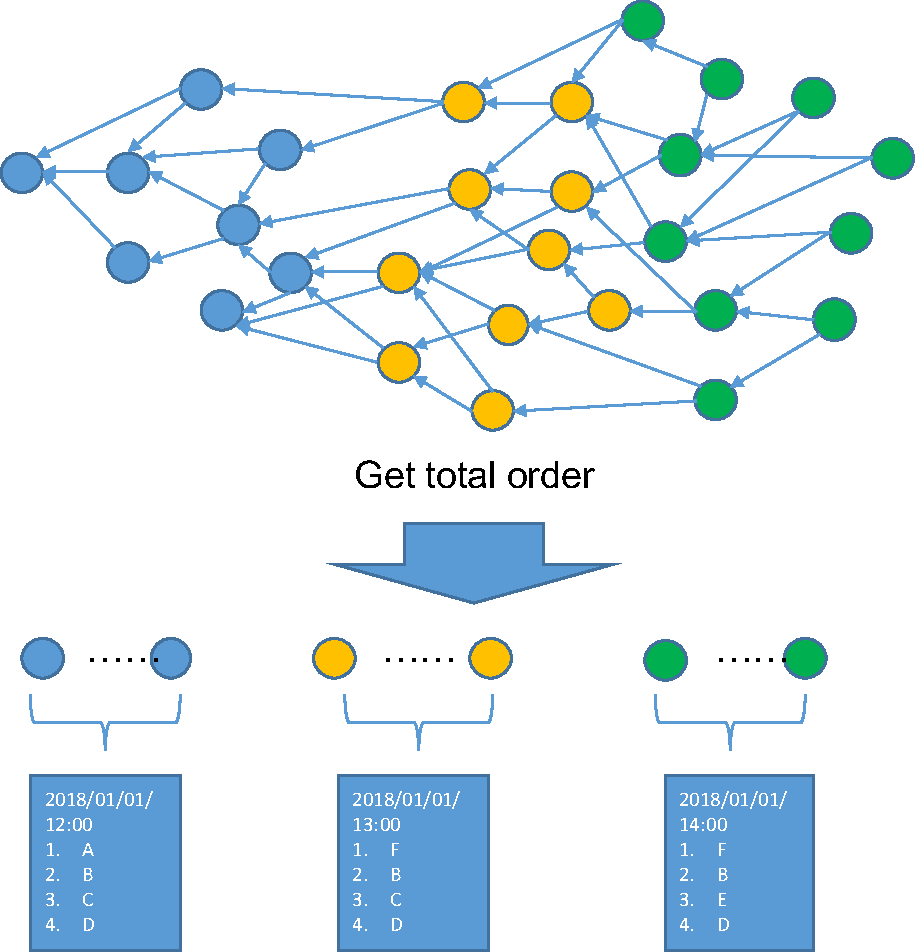
\includegraphics[width=0.45\textwidth]{figures/ranking.pdf}
                \caption{TRIAS ranking calculation based on the attestation information stored in StreamNet. Different color of blocks represent different periods.}
                \label{ranking}
        \end{center}
\end{figure}
